\section{Introduction}
\label{ref:intro}

This note presents two searches for beyond-the-standard model (BSM) physics in events
containing a leptonically-decaying Z boson, jets, and missing transverse energy. This
is an update of previous searches performed with 2011 data~\cite{ref:Zpaper,ref:EWKPAS}.
The search is based on a data sample of pp collisions collected at $\sqrt{s}=8$ TeV in 2012,
corresponding to an integrated luminosity of \lumi.

The production of Z bosons is expected in many BSM scenarios, for example supersymmetric (SUSY)
models. In SUSY models with neutralino lightest SUSY particle (LSP), Z bosons may be produced in the decays $\chi^0_2\to Z \chi^0_1$,
where $\chi^0_2$ is the second lightest neutralino and $\chi^0_1$ is
the lightest neutralino.
In models with gravitino LSP such as gauge-mediated SUSY breaking (GMSB) models, Z bosons may be produced via
$\chi^0_1\to Z \tilde{G}$, where $\tilde{G}$ is the gravitino. Such decays may occur either in the cascade
decays of the strongly-produced squarks and gluinos, or via direct production of the electroweak
charginos and neutralino. Examples of such processes (see Fig.~\ref{fig:diagrams}) are:

\begin{itemize}
\item strong production:      $pp\to\tilde{g}\tilde{g}\to (q\bar{q}\chi^0_2) (q\bar{q}\chi^0_2)\to(q\bar{q}Z\chi^0_1) (q\bar{q}Z\chi^0_1)\to$ ZZ + 4 jets + \MET
\item electroweak production: $pp\to\chi^\pm_1\chi^0_2\to (W \chi^0_1)(Z \chi^0_1) \to$ WZ + \MET
\end{itemize}

\begin{figure}[!h]
\begin{center}
\begin{tabular}{cc}
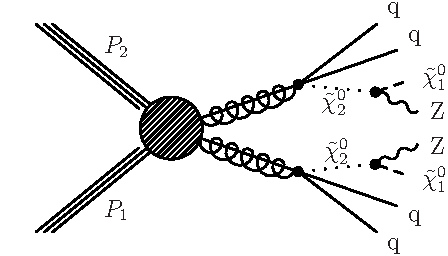
\includegraphics[width=0.4\textwidth]{plots/T5zz.pdf} &
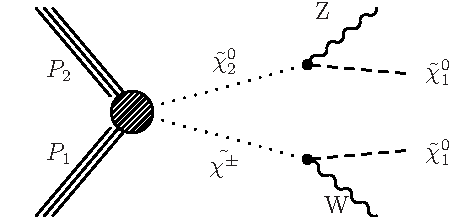
\includegraphics[width=0.4\textwidth]{plots/TChiwz.pdf} \\
\end{tabular}
\caption{
Examples of BSM physics signatures targeted in this search. In the left diagram, Z bosons are produced
in the cascade decays of the strongly-interacting gluinos. In the right diagram, a Z boson is produced
via direct production of the weakly-coupled charginos and neutralinos.
\label{fig:diagrams}
}
\end{center}
\end{figure}

We thus pursue two strategies. The first is an inclusive strategy which selects events with a Z$\to\ell\ell$ candidate,
at least two jets, and large \MET. This strategy is useful for targeting, e.g., the production of Z bosons in the 
cascade decays of strongly-interacting particles as depicted in Fig.~\ref{fig:diagrams} (left). In the second strategy,
we impose additional requirements which strongly suppress the backgrounds while retaining high efficiency for events
with Z bosons produced via direct production of the weakly-coupled charginos and neutralinos. 
These two strategies are referred to as the ``inclusive search'' and the ``targeted search,'' respectively.

After selecting events with jets and a $\Z\to\ell^+\ell^-$ ($\ell=e,\mu$) candidate,
the dominant background consists of SM \Z production accompanied by jets from initial-state radiation (\zjets).
The \MET\ in \zjets\ events arises primarily when jet energies are mismeasured.
The \zjets\ cross section is several orders of magnitude larger
than our signal, and the artificial \MET\ is not necessarily well reproduced in simulation.
Therefore, the critical prerequisite to a discovery of BSM physics in the $Z+\rm{jets}+\MET$ final state is 
to establish that a potential excess is not due to SM \zjets\ production accompanied by artificial 
\MET\ from jet mismeasurements. In this note, the \zjets\ background is estimated with the \MET templates technique,
in which the artificial \MET in \zjets events is modeled using a \gjets control sample.
The second background category consists of processes which produce leptons with uncorrelated flavor. 
These ``flavor-symmetric'' (FS) backgrounds, which are dominated by \ttbar\ but also contain WW, DY$\to\tau\tau$
and single top processes, are estimated using a data control sample of e$\mu$ events.
Additional backgrounds from WZ and ZZ production are estimated from MC, after validation of the MC modeling
of these processes using 3-lepton and 4-lepton data control samples.

